

\section{recall: sockets}

\begin{frame}{recall: sockets}
    \begin{itemize}
    \item open connection then \ldots \\
    \item read+write just like a terminal file
    \vspace{.5cm}
    \item doesn't look like individual messages
    \item ``connection abstraction''
    \end{itemize}
\end{frame}

\section{mailbox model}

\usetikzlibrary{arrows.meta,shapes.symbols,shapes.multipart}

\begin{frame}{mailbox model}
    \begin{itemize}
    \item \textit{mailbox} abstraction: send/receive messages
    \end{itemize}
    \begin{tikzpicture}
    \tikzset{
        >=Latex,
        comp box/.style={draw, thick, align=center, minimum width=1.5cm,minimum height=3cm},
        explain box/.style={draw=red,very thick, align=left},
        msg/.style={font=\small},
        cmd/.style={font=\small},
    }
        \node[comp box] (machine A) at (-6.5, 0) {machine \\ A};
        \node[draw,cloud,line width=1pt,minimum width=4cm,minimum height=1cm,aspect=3,
                alt=<2>{red,thick}] (network) at (0,0) {the network};
        \node[comp box] (machine B) at (6.5, 0) {machine \\ B};
        \draw[very thick,->] (machine A) -- (network) 
            node[alt=<1>{red},midway,above,msg] {B: ``Hello''}
            node[pos=0.0,below right,cmd] {Send(B, ``Hello'')};
        \draw[very thick,<-] (machine B) -- (network) 
            node[midway,above,msg] {B: ``Hello''}
            node[pos=0.0,below left,cmd] {Recv() = ``Hello''};
        % FIXME: hilite network: knows how to get message to particular place
            % note/show buffering at A/B
        \begin{visibleenv}<1>
            \node[explain box,anchor=north] at ([yshift=-.25cm]network.south) {
                A sends ``letter'' to B \\
                ``envelope'' tells network it's addressed to B \\
                data in this example: ``Hello''
            };
        \end{visibleenv}
        \begin{visibleenv}<2>
            \node[explain box,anchor=north] at ([yshift=-.25cm]network.south) {
                network does its \myemph{best} to get message to B
            };
        \end{visibleenv}
        \begin{visibleenv}<3->
            \node[anchor=south,draw,rectangle,rectangle split,rectangle split parts=5,rectangle split horizontal, inner sep=0.25mm] at ([yshift=.1cm]machine A.south) {
                ~~~
            };
        \end{visibleenv}
        \begin{visibleenv}<3>
            \node[explain box,anchor=north] at ([yshift=-.25cm]network.south) {
                queue (`outgoing mailbox') of messages \\
                from sending program \\
                waiting to be sent
            };
        \end{visibleenv}
        \begin{visibleenv}<4->
            \node[anchor=south,draw,rectangle,rectangle split,rectangle split parts=5,rectangle split horizontal,inner sep=0.25mm] at ([yshift=.1cm]machine B.south) {
                ~~~
            };
        \end{visibleenv}
        \begin{visibleenv}<4>
            \node[explain box,anchor=north] at ([yshift=-.25cm]network.south) {
                queue (`incoming mailbox') of messages \\
                not yet received by \\
                receiving program
            };
        \end{visibleenv}
    \end{tikzpicture}
\end{frame}

\begin{frame}{connections over mailboxes}
    \begin{itemize}
    \item real Internet: mailbox-style communication
    \item send ``letters'' (packets) to particular mailboxes
    \item have ``envelope'' (header) saying where they go
    \vspace{.5cm}
    \item ``best-effort''
    \item no gaurentee on order, when received
    \item no gaurentee on \textit{if} received
    \item sockets implemented on top of this
    \end{itemize}
\end{frame}


 % FIXME: wrong place?

\section{review: connection abstraction}

\usetikzlibrary{arrows.meta,shapes.symbols}
\begin{frame}{conections}
    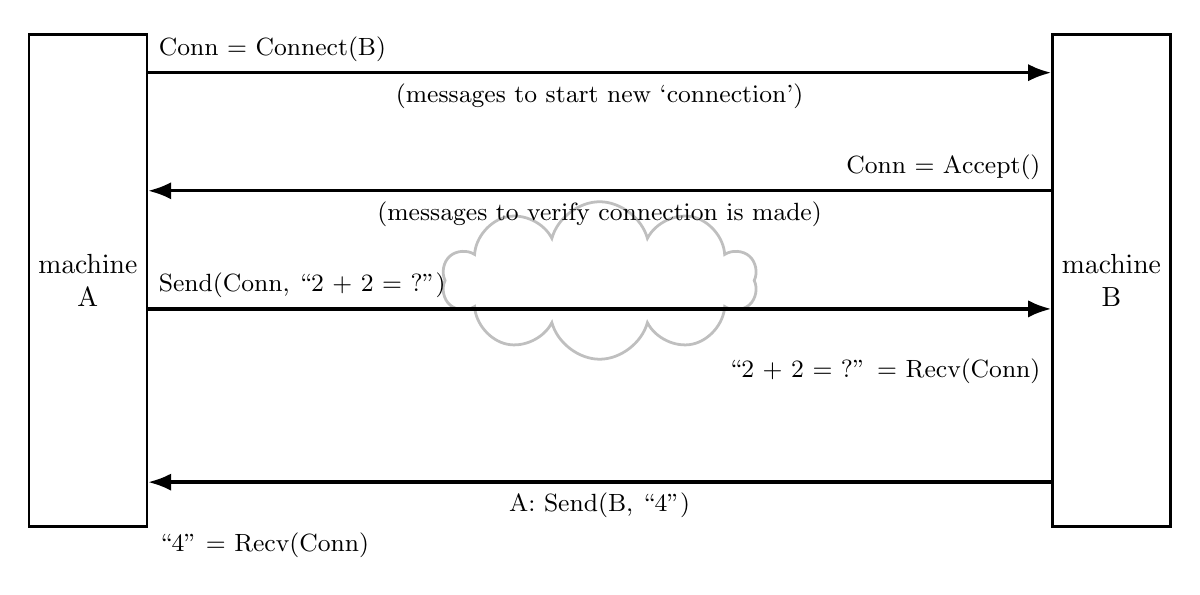
\begin{tikzpicture}
    \tikzset{
        >=Latex,
        comp box/.style={draw, thick, align=center, minimum width=1.5cm,minimum height=6.25cm},
        explain box/.style={draw=red,very thick, align=left},
        msg/.style={font=\small},
        cmd/.style={font=\small},
    }
        \node[comp box] (machine A) at (-6.5, 0) {machine \\ A};
        \node[draw,cloud,line width=1pt,minimum width=4cm,minimum height=2cm,aspect=3,opacity=0.25] (network) at (0,0) {~~};
        \node[comp box] (machine B) at (6.5, 0) {machine \\ B};
        \draw[very thick,->] ([yshift=-.5cm]machine A.north east) -- ([yshift=-.5cm]machine B.north west) 
            node[midway,below,msg] {(messages to start new `connection')}
            node[pos=0.0,above right,cmd] {Conn = Connect(B)};
        \draw[very thick,<-] ([yshift=-2cm]machine A.north east) -- ([yshift=-2cm]machine B.north west) 
            node[midway,below,msg] {(messages to verify connection is made)}
            node[pos=1.0,above left,cmd] {Conn = Accept()};
        \draw[very thick,->] ([yshift=-3.5cm]machine A.north east) -- ([yshift=-3.5cm]machine B.north west) 
            %node[midway,below,msg] {B: Send(A, ``2 + 2 = ?'')}
            node[pos=0.0,above right,cmd] {Send(Conn, ``2 + 2 = ?'')}
            node[pos=1.0,below left,cmd,yshift=-.5cm] {``2 + 2 = ?'' = Recv(Conn)};
        \draw[very thick,<-] ([yshift=-5.7cm]machine A.north east) -- ([yshift=-5.7cm]machine B.north west) 
            node[midway,below,msg] {A: Send(B, ``4'')}
            %node[pos=1.0,above left,cmd] {Send(Conn, ``4'')}
            node[pos=0.0,below right,cmd,yshift=-.5cm] {``4'' = Recv(Conn)};
    \end{tikzpicture}
\end{frame}



\section{layers preview}
\begin{frame}<1>[fragile,label=layerOverview]{networking layers}
\begin{tabular}{|l|l|p{6cm}|} \hline
application           & HTTP, SSH, SMTP, \ldots & {application-defined meanings}                                     \\ \hline
\myemph<6>{transport} & TCP, UDP, \ldots        & {reach correct program,\linebreak \myemph<2>{reliability/streams}} \\ \hline
\myemph<5>{network}   & IPv4, IPv6              & {reach correct machine}\linebreak(across networks)                 \\ \hline
\myemph<4>{link}      & Ethernet, Wi-Fi, \ldots & {coordinate shared wire/radio}                                     \\ \hline
physical              & Ethernet, Wi-Fi, \ldots & encode bits for wire/radio                                         \\ \hline
\end{tabular}
\end{frame}

\begin{frame}<1>[fragile,label=layerMsgNames]{layers terminology}
\begin{tabular}{|l|p{6cm}|l|} \hline
application & {application-defined meanings} & ~\\ \hline
transport & {reach correct program,\linebreak reliablity/streams} & segments/datagrams \\ \hline
network & {reach correct machine}\linebreak(across networks) & packets \\ \hline
link & {coordinate shared wire/radio} & frames \\ \hline
physical & encode bits for wire/radio & ~ \\ \hline
\end{tabular}
\end{frame}


\subsection{layer wrapping}
\begin{frame}{layer wrapping}
    \begin{itemize}
    \item upper layers usually implemented using lower layers
    \vspace{.5cm}
    \item example: implement reliable + large messages (transport layer) \\
        by sending multiple unreliable messages across networks (network layer)
    \item example: implement reaching machine across networks (network layer) \\
        by sending multiple messages on local networks (link layer)
    \end{itemize}
\end{frame}


\section{handling network failures}
\againframe<2>{layerOverview}

\begin{frame}<1>[label=netFailTypes]{network limitations/failures}
    \begin{itemize}
    \item \myemph<2>{messages lost}
    \item \myemph<3>{messages limited in size}
    \item \myemph<4>{messages delayed/reordered}
    \item \myemph<5>{messages corrupted}
    \end{itemize}
\end{frame}



\subsection{acknowledgments}
\againframe<2>{netFailTypes}
\usetikzlibrary{arrows.meta,shapes.misc,decorations.pathreplacing}

\begin{frame}{dealing with network message lost}
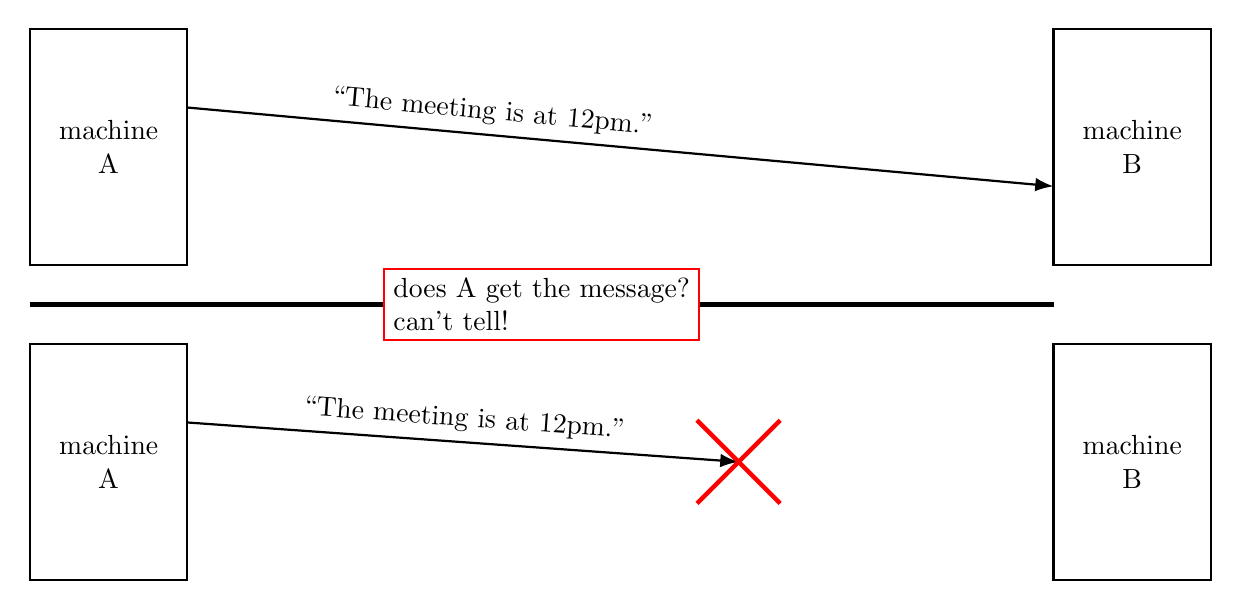
\begin{tikzpicture}
\tikzset{
    box/.style={draw,thick,minimum width=2cm},
    message/.style={draw,thick,-Latex},
    failure/.style={draw,ultra thick,red,cross out,minimum width=1cm,minimum height=1cm},
}
\begin{scope}
\draw[box] (0, 0) rectangle ++(2, -3) 
    node[midway,align=center] {machine\\ A};
\draw[box] (13, 0) rectangle ++(2, -3) 
    node[midway,align=center] {machine\\B};
\draw[message] (2, -1) -- (13, -2) node[pos=0.35, above, sloped] {``The meeting is at 12pm.''};
\end{scope}
\draw[ultra thick] (0, -3.5) -- ++ (13,0);
\begin{scope}[yshift=-4cm]
\draw[box] (0, 0) rectangle ++(2, -3) 
    node[midway,align=center] {machine\\A};
\draw[box] (13, 0) rectangle ++(2, -3) 
    node[midway,align=center] {machine\\B};
\draw[message] (2, -1) -- (9, -1.5) 
    node[pos=0.5,above,sloped] {``The meeting is at 12pm.''}
    node[failure] {};
\end{scope}
\node[draw=red,thick,fill=white,align=left] at (6.5, -3.5) {
    does A get the message? \\
    can't tell!
};
\end{tikzpicture}
\end{frame}

\begin{frame}{handling lost message: acknowledgements}
\begin{tikzpicture}
\tikzset{
    box/.style={thick},
    message/.style={draw,thick,-Latex},
    failure/.style={draw,ultra thick,red,cross out,minimum width=1cm,minimum height=1cm},
}
\begin{scope}
\draw[box] (0, 0) rectangle ++(2, -8) 
    node[midway,align=center] {machine\\A};
\draw[box] (13, 0) rectangle ++(2, -8) 
    node[midway,align=center] {machine\\B};
\draw[message] (2, -0.5) -- (13, -1) node[pos=0.35, above, sloped] {``The meeting is at 12pm.''};
\draw[message] (13, -1.5) -- (2, -2) node[pos=0.25, sloped,below] {Got it!};
\end{scope}
\end{tikzpicture}
\end{frame}

\begin{frame}{handling lost message}
\begin{tikzpicture}
\tikzset{
    box/.style={thick},
    message/.style={draw,thick,-Latex},
    failure/.style={draw,ultra thick,red,cross out,minimum width=1cm,minimum height=1cm},
}
\draw[box] (0, 0) rectangle ++(2, -8) 
    node[midway,align=center] {machine\\A};
\draw[box] (13, 0) rectangle ++(2, -8) 
    node[midway,align=center] {machine\\B};
%\draw[message] (2, -0.5) -- (13, -1) node[pos=0.35, above, sloped] {``The meeting is at 12pm.''};
\draw[message] (2, -0.5) -- (9, -1) 
    node[pos=0.5,above,sloped] {``The meeting is at 12pm.''}
    node[failure] {};
\begin{visibleenv}<2->
\draw[decorate,decoration={brace}] (2.1, -1) -- (2.1, -3) 
    node[midway,right,align=left] {
        ``timeout'' \\
        A doesn't get reply \\
        after waiting too long
    };
\end{visibleenv}
\begin{visibleenv}<3->
\draw[message] (2, -4) -- (13, -5) node[pos=0.35, above, sloped] {``The meeting is at 12pm.''};
\draw[message] (13, -5.5) -- (2, -6) node[pos=0.5, sloped,below] {Got it!};
\end{visibleenv}
\end{tikzpicture}
\end{frame}

\begin{frame}{lost acknowledgements}
\begin{tikzpicture}
\tikzset{
    box/.style={thick},
    message/.style={draw,thick,-Latex},
    failure/.style={draw,ultra thick,red,cross out,minimum width=1cm,minimum height=1cm},
}
\draw[box] (0, 0) rectangle ++(2, -8) 
    node[midway,align=center] {machine\\A};
\draw[box] (13, 0) rectangle ++(2, -8) 
    node[midway,align=center] {machine\\B};
\draw[message] (2, -0.5) -- (13, -1) node[pos=0.35, above, sloped] {``The meeting is at 12pm.''};
\draw[message] (13, -1.5) -- (6.5, -1.75) node[pos=0.5, sloped,below] {Got it!}
    node[failure] {};
\begin{visibleenv}<3->
\draw[message] (2, -3.5) -- (13, -4) node[pos=0.35, above, sloped] {``The meeting is at 12pm.''};
\draw[message] (13, -4.5) -- (2, -5) node[pos=0.5, sloped,below] {Got it!};
\end{visibleenv}
\begin{visibleenv}<2>
\node[draw=red,thick,fill=white,align=left] at (6.5, -6.5) {
    A's going to need to resend this message! \\
    Can't tell it really was received!
};
\end{visibleenv}
\begin{visibleenv}<3>
\node[draw=red,thick,fill=white,align=left] at (6.5, -6.5) {
    B needs to handle receiving message twice! \\
    Sockets: you only get a copy of the data once.
};
\end{visibleenv}
\end{tikzpicture}
\end{frame}


\begin{frame}{delayed acknowledgements}
\begin{tikzpicture}
\tikzset{
    box/.style={thick},
    message/.style={draw,thick,-Latex},
    failure/.style={draw,ultra thick,red,cross out,minimum width=1cm,minimum height=1cm},
}
\draw[box] (0, 0) rectangle ++(2, -8) 
    node[midway,align=center] {machine\\A};
\draw[box] (13, 0) rectangle ++(2, -8) 
    node[midway,align=center] {machine\\B};
\draw[message] (2, -0.5) -- (13, -1) node[pos=0.35, above, sloped] {``The meeting is at 12pm.''};
\draw[message] (13, -1.5) -- (2, -5) node[pos=0.25, sloped,below] {Got it!};
\draw[decorate,decoration={brace}] (2.1, -1) -- (2.1, -3) 
    node[midway,right,align=left] {
        ``timeout''
    };
\begin{visibleenv}<3->
\draw[message] (2, -3.5) -- (13, -4) node[pos=0.35, above, sloped] {``The meeting is at 12pm.''};
\draw[message] (13, -4.5) -- (2, -6) node[pos=0.5, sloped,below] {Got it!};
\end{visibleenv}
\begin{visibleenv}<3>
\node[draw=red,thick,fill=white,align=left] at (8, -6.5) {
    B can't tell that first acknowledgment wasn't lost
};
\end{visibleenv}
\end{tikzpicture}
\end{frame}

\subsubsection{exercise: lost acks}
\begin{frame}{exercise: lost acknowledgement}
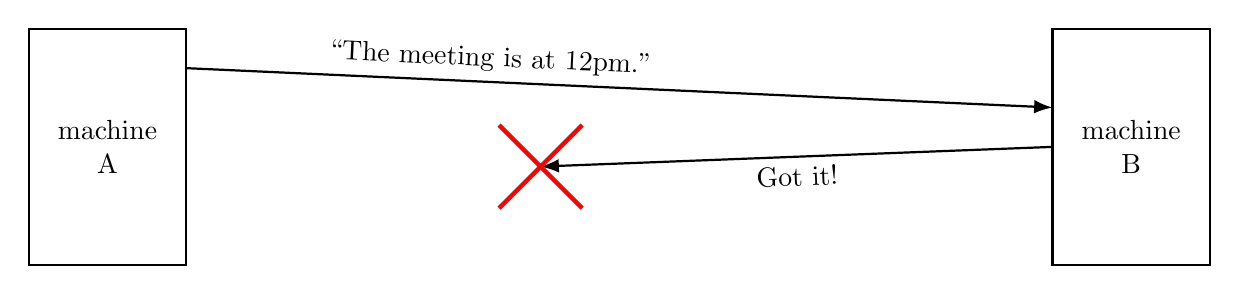
\begin{tikzpicture}
\tikzset{
    box/.style={thick},
    message/.style={draw,thick,-Latex},
    failure/.style={draw,ultra thick,red,cross out,minimum width=1cm,minimum height=1cm},
}
\draw[box] (0, 0) rectangle ++(2, -3) 
    node[midway,align=center] {machine\\A};
\draw[box] (13, 0) rectangle ++(2, -3) 
    node[midway,align=center] {machine\\B};
\draw[message] (2, -0.5) -- (13, -1) node[pos=0.35, above, sloped] {``The meeting is at 12pm.''};
\draw[message] (13, -1.5) -- (6.5, -1.75) node[pos=0.5, sloped,below] {Got it!}
    node[failure] {};
\end{tikzpicture}
exercise: how to fix this?
\begin{tabular}{ll}
A. & machine A needs to send ``Got `got it!' '' \\
B. & machine B should resend ``Got it!'' on its own \\
C. & machine A should resend the original message on its own \\
D. & none of these \\
\end{tabular}
\end{frame}

\begin{frame}<0>[label=lostAckExExplain]{answers}
\begin{itemize}
\item send ``Got `got it!' ''?
    \begin{itemize}
    \item same problem: Now send `Got Got Got it'?
    \end{itemize}
\item resend ``Got it!'' own its own?
    \begin{itemize}
    \item how many times? --- B doesn't have that info
    \end{itemize}
\item resend original message?
    \begin{itemize}
    \item yes!
    \item as far as machine A can see, \textit{exact same situation} as losing original message
    \end{itemize}
\end{itemize}
\end{frame}

\iftoggle{heldback}{}{
    \againframe<1>{lostAckExExplain}
}


\subsubsection{solution: lost acks}
\iftoggle{heldback}{}{

\begin{frame}{lost acknowledgements}
\begin{tikzpicture}
\tikzset{
    box/.style={thick},
    message/.style={draw,thick,-Latex},
    failure/.style={draw,ultra thick,red,cross out,minimum width=1cm,minimum height=1cm},
}
\draw[box] (0, 0) rectangle ++(2, -8) 
    node[midway,align=center] {machine\\A};
\draw[box] (13, 0) rectangle ++(2, -8) 
    node[midway,align=center] {machine\\B};
\draw[message] (2, -0.5) -- (13, -1) node[pos=0.35, above, sloped] {``The meeting is at 12pm.''};
\draw[message] (13, -1.5) -- (6.5, -1.75) node[pos=0.5, sloped,below] {Got it!}
    node[failure] {};
\begin{visibleenv}<3->
\draw[message] (2, -3.5) -- (13, -4) node[pos=0.35, above, sloped] {``The meeting is at 12pm.''};
\draw[message] (13, -4.5) -- (2, -5) node[pos=0.5, sloped,below] {Got it!};
\end{visibleenv}
\begin{visibleenv}<2>
\node[draw=red,thick,fill=white,align=left] at (6.5, -6.5) {
    A's going to need to resend this message! \\
    Can't tell it really was received!
};
\end{visibleenv}
\begin{visibleenv}<3>
\node[draw=red,thick,fill=white,align=left] at (6.5, -6.5) {
    B needs to handle receiving message twice! \\
    Sockets: you only get a copy of the data once.
};
\end{visibleenv}
\end{tikzpicture}
\end{frame}
}
\subsubsection{delayed acks}
\againframe<3>{netFailTypes}

\begin{frame}{delayed message}
\begin{tikzpicture}
\tikzset{
    box/.style={thick},
    message/.style={draw,thick,-Latex},
    failure/.style={draw,ultra thick,red,cross out,minimum width=1cm,minimum height=1cm},
}
\draw[box] (0, 0) rectangle ++(2, -8) 
    node[midway,align=center] {machine\\A};
\draw[box] (13, 0) rectangle ++(2, -8) 
    node[midway,align=center] {machine\\B};
\draw[message] (2, -0.5) -- (13, -4.5) node[pos=0.35, above, sloped] {``The meeting is at 12pm.''};
\draw[message] (13, -4.5) -- (2, -5) node[pos=0.25, sloped,below] {Got it!};
\draw[decorate,decoration={brace}] (2.1, -1) -- (2.1, -3) 
    node[midway,right,align=left] {
        ``timeout''
    };
\begin{visibleenv}<3->
\draw[message] (2, -3.5) -- (13, -5) node[pos=0.35, above, sloped] {``The meeting is at 12pm.''};
\draw[message] (13, -5.5) -- (2, -6) node[pos=0.5, sloped,below] {Got it!};
\end{visibleenv}
\begin{visibleenv}<3>
\node[draw=red,thick,fill=white,align=left] at (8, -7) {
    B resends, can't tell message is just slow
};
\end{visibleenv}
\end{tikzpicture}
\end{frame}


\begin{frame}{delayed acknowledgements}
\begin{tikzpicture}
\tikzset{
    box/.style={thick},
    message/.style={draw,thick,-Latex},
    failure/.style={draw,ultra thick,red,cross out,minimum width=1cm,minimum height=1cm},
}
\draw[box] (0, 0) rectangle ++(2, -8) 
    node[midway,align=center] {machine\\A};
\draw[box] (13, 0) rectangle ++(2, -8) 
    node[midway,align=center] {machine\\B};
\draw[message] (2, -0.5) -- (13, -1) node[pos=0.35, above, sloped] {``The meeting is at 12pm.''};
\draw[message] (13, -1.5) -- (2, -5) node[pos=0.25, sloped,below] {Got it!};
\draw[decorate,decoration={brace}] (2.1, -1) -- (2.1, -3) 
    node[midway,right,align=left] {
        ``timeout''
    };
\begin{visibleenv}<3->
\draw[message] (2, -3.5) -- (13, -4) node[pos=0.35, above, sloped] {``The meeting is at 12pm.''};
\draw[message] (13, -4.5) -- (2, -6) node[pos=0.5, sloped,below] {Got it!};
\end{visibleenv}
\begin{visibleenv}<3>
\node[draw=red,thick,fill=white,align=left] at (8, -6.5) {
    B can't tell that first acknowledgment wasn't lost
};
\end{visibleenv}
\end{tikzpicture}
\end{frame}



\subsection{splitting into multiple}
\againframe<4>{netFailTypes}
\usetikzlibrary{arrows.meta,decorations.pathreplacing,shapes.misc}

\begin{frame}{splitting messages: try 1}
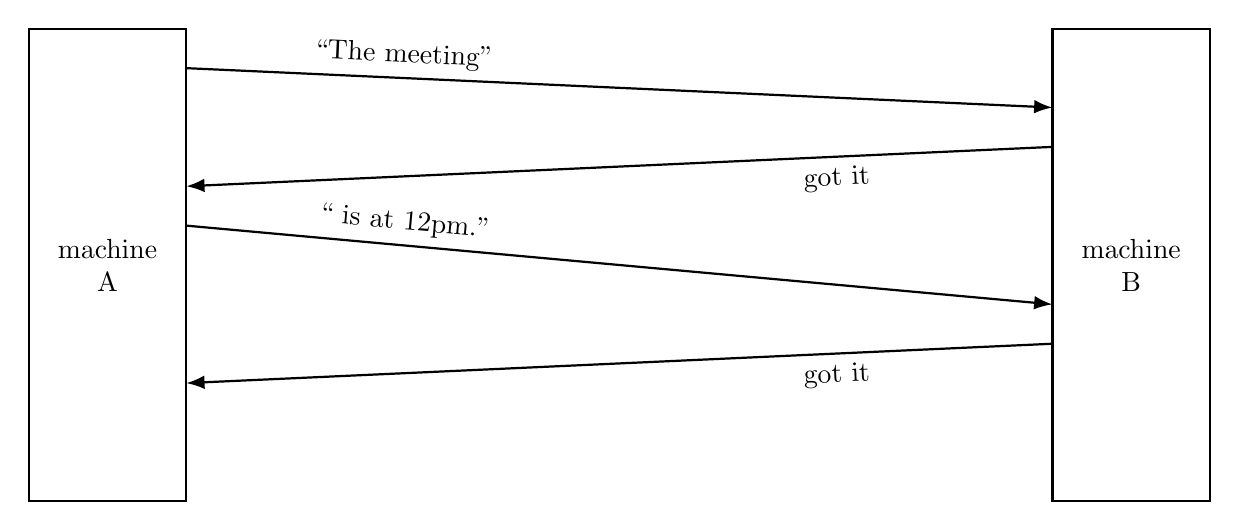
\begin{tikzpicture}
\tikzset{
    box/.style={thick},
    message/.style={draw,thick,-Latex},
    failure/.style={draw,ultra thick,red,cross out,minimum width=1cm,minimum height=1cm},
}
\begin{scope}
\draw[box] (0, 0) rectangle ++(2, -6) 
    node[midway,align=center] {machine\\A};
\draw[box] (13, 0) rectangle ++(2, -6) 
    node[midway,align=center] {machine\\B};
\draw[message] (2, -0.5) -- (13, -1) node[pos=0.25, above, sloped] {``The meeting''};
\draw[message] (13, -1.5) -- (2, -2) node[pos=0.25, sloped,below] {got it};
\draw[message] (2, -2.5) -- (13, -3.5) node[pos=0.25, above, sloped] {`` is at 12pm.''};
\draw[message] (13, -4) -- (2, -4.5) node[pos=0.25, sloped,below] {got it};
\end{scope}
\end{tikzpicture}
reconstructed message: \\
The meeting is at 12pm.
\end{frame}


\begin{frame}{splitting messages: try 1 --- problem}
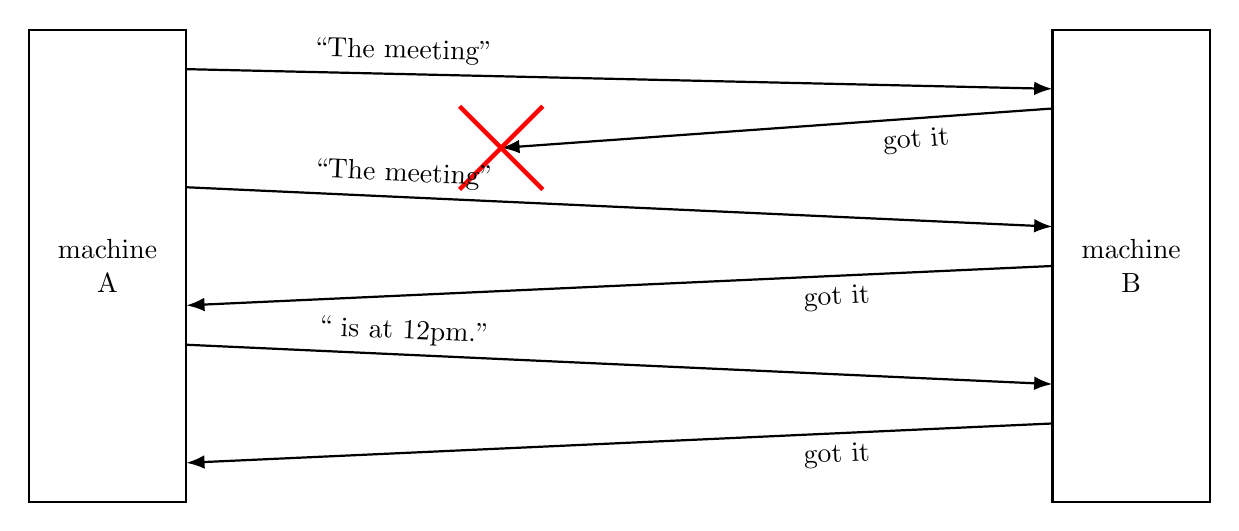
\begin{tikzpicture}
\tikzset{
    box/.style={thick},
    message/.style={draw,thick,-Latex},
    failure/.style={draw,ultra thick,red,cross out,minimum width=1cm,minimum height=1cm},
}
\begin{scope}
\draw[box] (0, 0) rectangle ++(2, -6) 
    node[midway,align=center] {machine\\A};
\draw[box] (13, 0) rectangle ++(2, -6) 
    node[midway,align=center] {machine\\B};
\draw[message] (2, -0.5) -- (13, -0.75) node[pos=0.25, above, sloped] {``The meeting''};
\draw[message] (13, -1) -- (6, -1.5) node[pos=0.25, sloped,below] {got it} node[failure] {};
\draw[message] (2, -2) -- (13, -2.5) node[pos=0.25, above, sloped] {``The meeting''};
\draw[message] (13, -3) -- (2, -3.5) node[pos=0.25, sloped,below] {got it};
\draw[message] (2, -4) -- (13, -4.5) node[pos=0.25, above, sloped] {`` is at 12pm.''};
\draw[message] (13, -5) -- (2, -5.5) node[pos=0.25, sloped,below] {got it};
\end{scope}
\end{tikzpicture}
reconstructed message: \\
The meetingThe meeting is at 12pm.
\end{frame}

\begin{frame}{splitting messages: try 2}
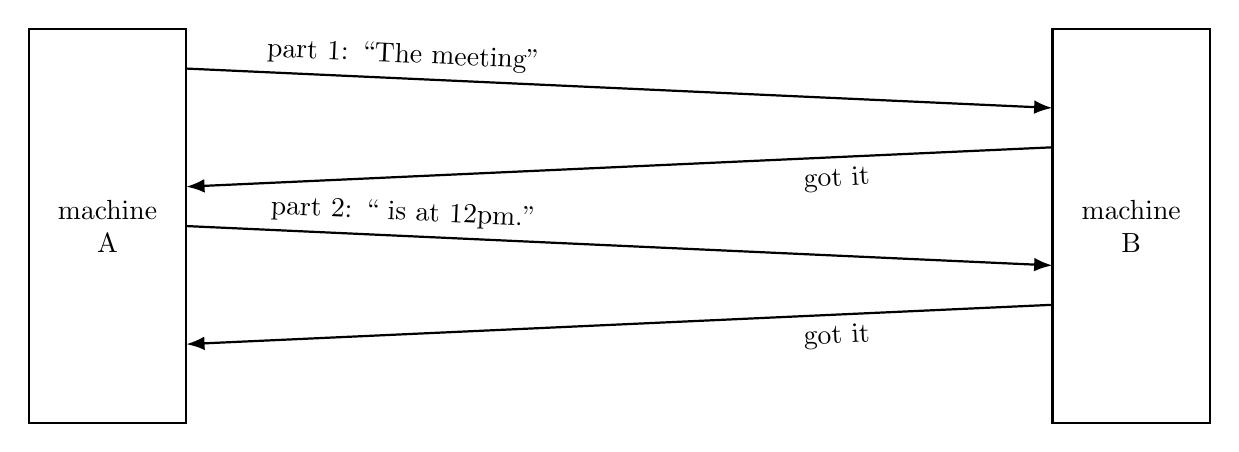
\begin{tikzpicture}
\tikzset{
    box/.style={thick},
    message/.style={draw,thick,-Latex},
    failure/.style={draw,ultra thick,red,cross out,minimum width=1cm,minimum height=1cm},
}
\begin{scope}
\draw[box] (0, 0) rectangle ++(2, -5) 
    node[midway,align=center] {machine\\A};
\draw[box] (13, 0) rectangle ++(2, -5) 
    node[midway,align=center] {machine\\B};
\draw[message] (2, -0.5) -- (13, -1) node[pos=0.25, above, sloped] {part 1: ``The meeting''};
\draw[message] (13, -1.5) -- (2, -2) node[pos=0.25, sloped,below] {got it};
\draw[message] (2, -2.5) -- (13, -3) node[pos=0.25, above, sloped] {part 2: `` is at 12pm.''};
\draw[message] (13, -3.5) -- (2, -4) node[pos=0.25, sloped,below] {got it};
\end{scope}
\end{tikzpicture}
reconstructed message: \\
The meeting is at 12pm.
\end{frame}

\begin{frame}{splitting messages: try 2 --- missed ack}
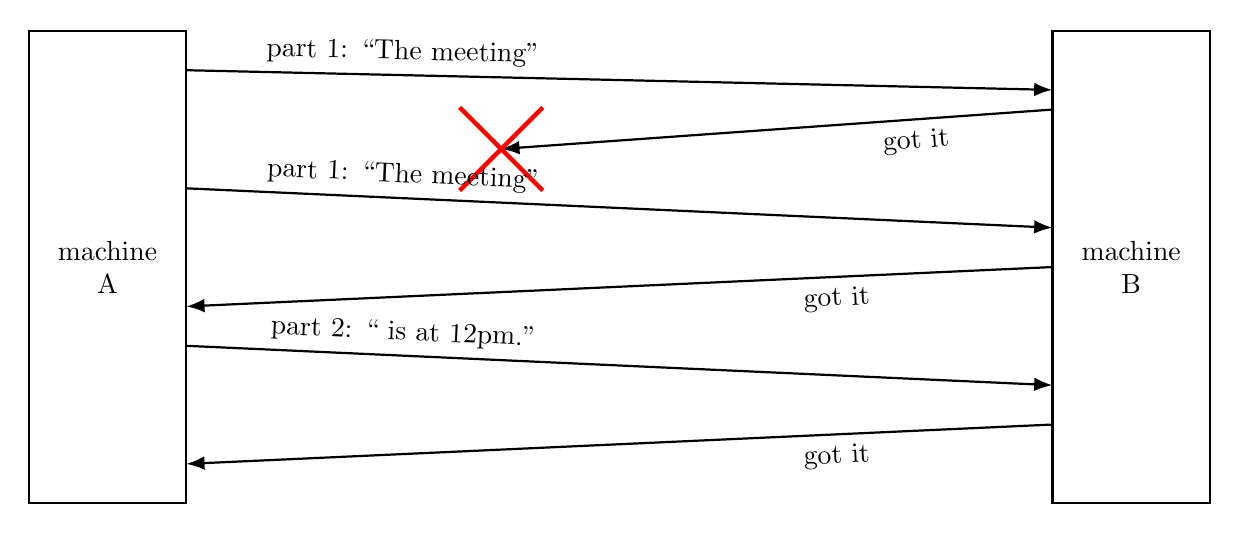
\begin{tikzpicture}
\tikzset{
    box/.style={thick},
    message/.style={draw,thick,-Latex},
    failure/.style={draw,ultra thick,red,cross out,minimum width=1cm,minimum height=1cm},
}
\begin{scope}
\draw[box] (0, 0) rectangle ++(2, -6) 
    node[midway,align=center] {machine\\A};
\draw[box] (13, 0) rectangle ++(2, -6) 
    node[midway,align=center] {machine\\B};
\draw[message] (2, -0.5) -- (13, -0.75) node[pos=0.25, above, sloped] {part 1: ``The meeting''};
\draw[message] (13, -1) -- (6, -1.5) node[pos=0.25, sloped,below] {got it} node[failure] {};
\draw[message] (2, -2) -- (13, -2.5) node[pos=0.25, above, sloped] {part 1: ``The meeting''};
\draw[message] (13, -3) -- (2, -3.5) node[pos=0.25, sloped,below] {got it};
\draw[message] (2, -4) -- (13, -4.5) node[pos=0.25, above, sloped] {part 2: `` is at 12pm.''};
\draw[message] (13, -5) -- (2, -5.5) node[pos=0.25, sloped,below] {got it};
\end{scope}
\end{tikzpicture}
reconstructed message: \\
The meeting is at 12pm.
\end{frame}

\begin{frame}{splitting messages: try 2 --- problem}
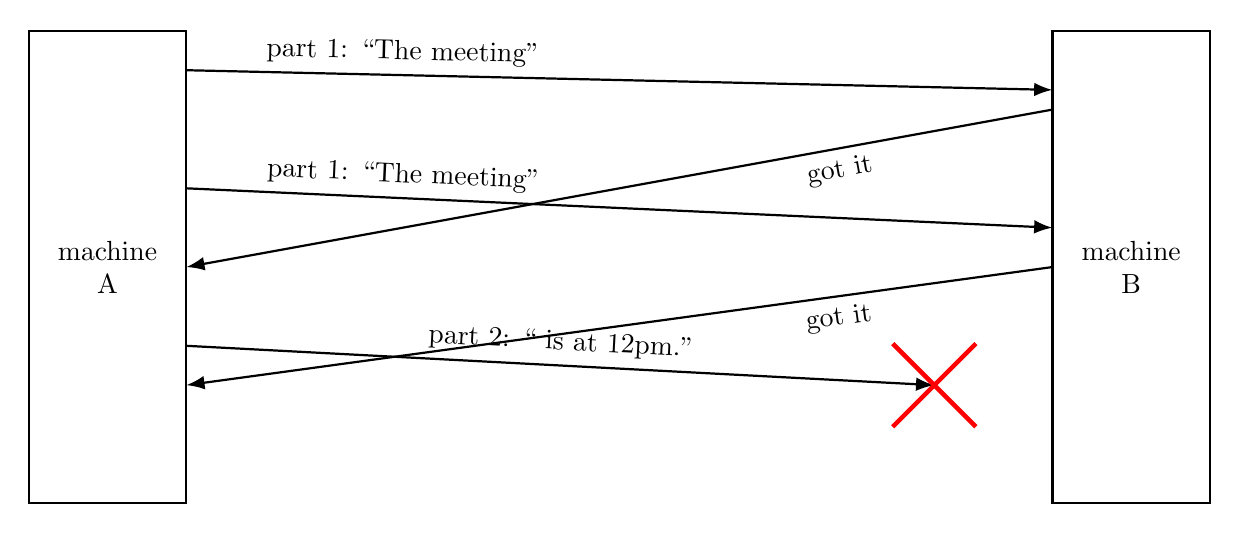
\begin{tikzpicture}
\tikzset{
    box/.style={thick},
    message/.style={draw,thick,-Latex},
    failure/.style={draw,ultra thick,red,cross out,minimum width=1cm,minimum height=1cm},
}
\begin{scope}
\draw[box] (0, 0) rectangle ++(2, -6) 
    node[midway,align=center] {machine\\A};
\draw[box] (13, 0) rectangle ++(2, -6) 
    node[midway,align=center] {machine\\B};
\draw[message] (2, -0.5) -- (13, -0.75) node[pos=0.25, above, sloped] {part 1: ``The meeting''};
\draw[message] (13, -1) -- (2, -3) node[pos=0.25, sloped,below] {got it};
\draw[message] (2, -2) -- (13, -2.5) node[pos=0.25, above, sloped] {part 1: ``The meeting''};
\draw[message] (13, -3) -- (2, -4.5) node[pos=0.25, sloped,below] {got it};
\draw[message] (2, -4) -- (11.5, -4.5) node[pos=0.5, above, sloped] {part 2: `` is at 12pm.''}
    node[failure] {};
\end{scope}
\end{tikzpicture}
A thinks: part 1 + part 2 acknowleged!
\end{frame}

\begin{frame}{splitting messages: version 3}
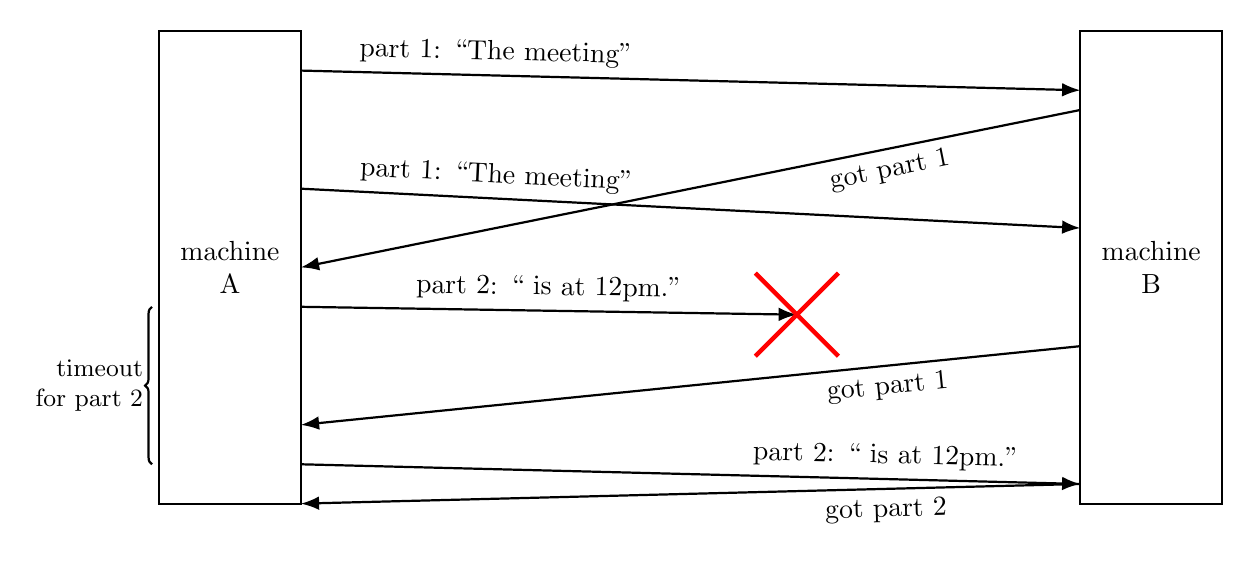
\begin{tikzpicture}
\tikzset{
    box/.style={thick},
    message/.style={draw,thick,-Latex},
    failure/.style={draw,ultra thick,red,cross out,minimum width=1cm,minimum height=1cm},
}
\begin{scope}[xshift=1cm,x=0.9cm]
\draw[box] (0, 0) rectangle ++(2, -6) 
    node[midway,align=center] {machine\\A};
\draw[box] (13, 0) rectangle ++(2, -6) 
    node[midway,align=center] {machine\\B};
\draw[message] (2, -0.5) -- (13, -0.75) node[pos=0.25, above, sloped] {part 1: ``The meeting''};
\draw[message] (13, -1) -- (2, -3) node[pos=0.25, sloped,below] {got \myemph{part 1}};
\draw[message] (2, -2) -- (13, -2.5) node[pos=0.25, above, sloped] {part 1: ``The meeting''};
\draw[message] (13, -4) -- (2, -5) node[pos=0.25, sloped,below] {got \myemph{part 1}};
\draw[message] (2, -3.5) -- (9, -3.6) node[pos=0.5, above, sloped] {part 2: `` is at 12pm.''}
    node[failure] {};
\draw[thick,decorate,decoration={brace,mirror}] (-0.1, -3.5) -- (-0.1, -5.5) node[inner sep=1mm,font=\small,align=right,midway,left] {timeout\\\myemph{for part 2}};
\draw[message] (2, -5.5) -- (13, -5.75) node[pos=0.75, above, sloped] {part 2: `` is at 12pm.''};
\draw[message] (13, -5.75) -- (2, -6) node[pos=0.25, below, sloped] {got \myemph{part 2}};
\end{scope}
\end{tikzpicture}
\end{frame}


    % FIXME: exercise
        % acknowledge only last
        % partial acknowledgments

\subsection{checksums}
\againframe<5>{netFailTypes}
\begin{frame}{message corrupted}
\begin{itemize}
\item instead of sending ``message''
\vspace{.5cm}
\item say Hash(``message'') = 0xABCDEF12
\item then send ``0xABCDEF12,message''
\vspace{.5cm}
\item when receiving, recompute hash
\item pretend message lost if does not match
\end{itemize}
\end{frame}

\begin{frame}{``checksum''}
\begin{itemize}
\item these hashes commonly called ``checksums''
\item in UDP/TCP, hash function: treat bytes of messages as array of integers; then add integers together
\end{itemize}
\end{frame}

    % FIXME: exercise: 

\subsection{aside: going faster}
\begin{frame}{going faster}
    \begin{itemize}
    \item so far: send one message, wait for acknowledgment
    \vspace{.5cm}
    \item very slow!
    \item instead, can send a bunch of parts and get them acknowledged together
    % \item need to do \textit{congestion control} to avoid overloading network
    \end{itemize}
\end{frame}

\usetikzlibrary{arrows.meta,decorations.pathreplacing,shapes.misc}

\begin{frame}{transmission window (ex: size 4)}
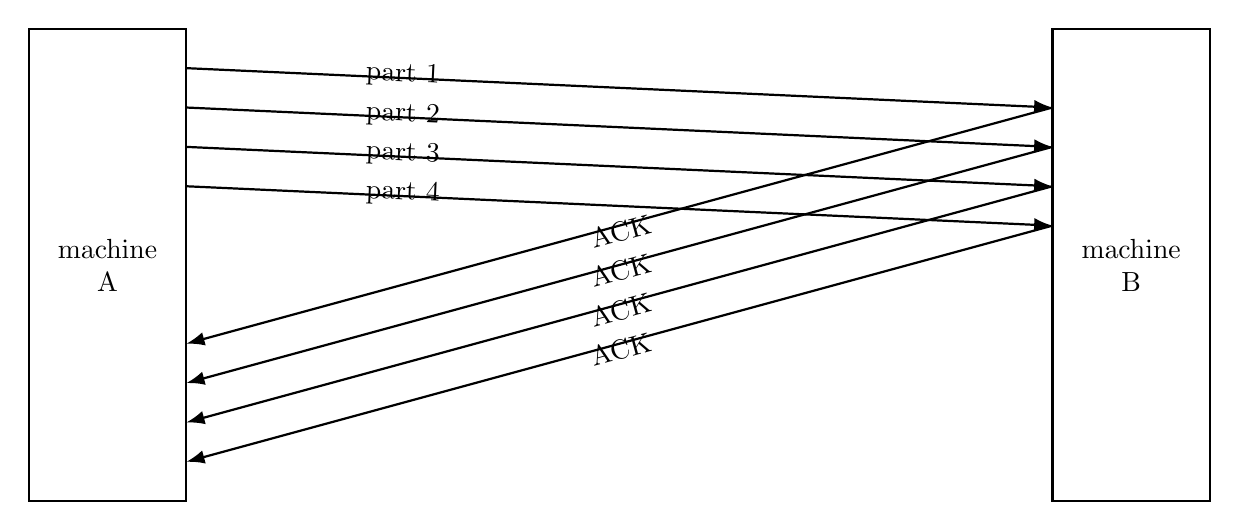
\begin{tikzpicture}
\tikzset{
    box/.style={thick},
    message/.style={draw,thick,-Latex},
    failure/.style={draw,ultra thick,red,cross out,minimum width=1cm,minimum height=1cm},
}
\begin{scope}
\draw[box] (0, 0) rectangle ++(2, -6)
    node[midway,align=center] {machine\\A};
\draw[box] (13, 0) rectangle ++(2, -6)
    node[midway,align=center] {machine\\B};
\draw[message] (2, -0.5) -- (13, -1.0) node[pos=0.25, above=-7pt, sloped] {part 1};
\draw[message] (2, -1.0) -- (13, -1.5) node[pos=0.25, above=-7pt, sloped] {part 2};
\draw[message] (2, -1.5) -- (13, -2.0) node[pos=0.25, above=-7pt, sloped] {part 3};
\draw[message] (2, -2.0) -- (13, -2.5) node[pos=0.25, above=-7pt, sloped] {part 4};
\draw[message] (13, -1.0) -- (2, -4.0) node[pos=0.5, sloped, below=-5pt] {ACK};
\draw[message] (13, -1.5) -- (2, -4.5) node[pos=0.5, sloped, below=-5pt] {ACK};
\draw[message] (13, -2.0) -- (2, -5.0) node[pos=0.5, sloped, below=-5pt] {ACK};
\draw[message] (13, -2.5) -- (2, -5.5) node[pos=0.5, sloped, below=-5pt] {ACK};
\end{scope}
\end{tikzpicture}
Send a \textit{window} of parts speculatively, then wait for ACKs.
\end{frame}


\section{layers, revisited}
\againframe<3>{layerOverview}

\begin{frame}{more than four layers?}
    \begin{itemize}
    \item sometimes more layers above `application'
    \item e.g. HTTPS:
        \begin{itemize}
        \item HTTP (app layer) on TLS (another app layer) on TCP (network) on \ldots
        \end{itemize}
    \item e.g. DNS over HTTPS:
        \begin{itemize}
        \item DNS (app layer) on HTTP on on TLS on TCP on \ldots
        \end{itemize}
    \item e.g. SFTP:
        \begin{itemize}
        \item SFTP (app layer??) on SSH (another app layer) on TCP on \ldots
        \end{itemize}
    \item e.g. HTTP over OpenVPN:
        \begin{itemize}
        \item HTTP on TCP on IP on OpenVPN on UDP on different IP on \ldots
        \end{itemize}
    \end{itemize}
\end{frame}


\section{addresses versus names}
\usetikzlibrary{arrows.meta,calc,positioning,shapes.callouts,shapes.symbols}

\begin{frame}{names and addresses}
\small
\begin{tabular}{l|l}
\textbf{name} & \textbf{address} \\\hline
\large\myemph{logical identifier} & \large\myemph{location/how to locate} \\
~ & ~ \\
variable \texttt{counter} & memory address \texttt{0x7FFF9430} \\ 
~ & ~ \\
DNS name \texttt{www.virginia.edu} & IPv4 address \texttt{128.143.22.36} \\
DNS name \texttt{mail.google.com} & IPv4 address \texttt{216.58.217.69} \\
DNS name \texttt{mail.google.com} & IPv6 address \fontsize{10}{11}\selectfont\texttt{2607:f8b0:4004:80b::2005} \\
    DNS name \fontsize{10}{11}\selectfont\texttt{reiss-t3620.cs.virginia.edu} & IPv4 address \texttt{128.143.67.91} \\
    DNS name \fontsize{10}{11}\selectfont\texttt{reiss-t3620.cs.virginia.edu} & MAC address \texttt{18:66:da:2e:7f:da} \\
~ & ~ \\
service name \texttt{https} & port number \texttt{443} \\
service name \texttt{ssh} & port number \texttt{22} \\
\end{tabular}
\end{frame}



\section{a frame example}
\againframe<4>{layerOverview}
\usetikzlibrary{decorations.pathreplacing,fit,matrix}
\begin{frame}{an Ethernet frame}
\begin{tikzpicture}
\tikzset{
    small label/.style={font=\small},
    box/.style={thick},
}
\matrix[tight matrix no line,
    nodes={font=\tt\small\strut,text width=0.7cm},
] {
|[alias=destMacStart]| 4c \& cc \& 6a \& ba \& 1c \& |[alias=destMacEnd]| b9 \& 
|[alias=sourceMacStart]| d8 \& 07 \& b6 \& d9 \& ae \& |[alias=sourceMacEnd]| 50 \&
|[alias=etherTypeStart]| 08 \& |[alias=etherTypeEnd]| 00 \\[1cm]
|[alias=ipTypeHLen,alias=ipHeadStart]| \alt<2->{\setlength{\fboxsep}{0pt}\colorbox{orange!20}{4}}{4}5 \& 
|[alias=ipDiffServ]| 00 \& 
|[alias=ipLenStart]| 00 \& |[alias=ipLenEnd]| 60\&
|[alias=ipIdStart]| db \& |[alias=ipIdEnd]| 89 \&
|[alias=ipFlagsAndFragStart]| 40 \& |[alias=ipFlagsAndFragEnd]| 00 \& 
|[alias=ipTTL]| f2 \& 
|[alias=ipProto]| 06 \& 
|[alias=ipChkSumSt]| cf \& |[alias=ipChkSumEnd]| cd \&
|[alias=ipSrcStart]| 34 \& 60 \& e6 \& |[alias=ipSrcEnd,alias=ipFirstLine]| a2 \\[1cm]
|[alias=ipDstStart]| c0 \& a8 \& 01 \& |[alias=ipDstEnd]| 95 \&
|[alias=tcpHeadStart,alias=srcPortStart]| 01 \& |[alias=srcPortEnd]| bb \& |[alias=dstPortStart]| aa \& |[alias=dstPortEnd]| c4 \& |[alias=seqNumStart]| 40 \& 2b \& d6 \& |[alias=seqNumEnd]| 46 \& 
    |[alias=ackNumStart]| 7c \& 9d \& 15 \& |[alias=tcpHeadFirstLine,alias=ackNumEnd]| e4 \\[.7cm] 
|[alias=tcpSecondLine,alias=tcpFlagsStart]| 80 \& |[alias=tcpFlagsEnd]| 18 \& |[alias=tcpWinStart]| 40 \& |[alias=tcpWinEnd]| 02 \& 
|[alias=checkSumStart]| 65 \& |[alias=checkSumEnd]| fe \& |[alias=urgentStart]| 00 \& |[alias=urgentEnd]| 00 \&
|[alias=tcpOptStart]| 01 \& 01 \& 08 \& 0a \& 03 \& 83 \& 98 \& 62 \\[.7cm]
19 \& 70 \& 27 \& |[alias=tcpOptEnd]| 9e \& |[alias=tcpDataStart]| 17 \& 03 \& 03 \& 00 \& 27 \& 00 \& 00 \& 00 \& 00 \& 00 \& 00 \& |[alias=tcpDataFirstLine]| 00 \\
|[alias=tcpDataSecondLine]| c8 \& b9 \& ab \& 81 \& 50 \& e0 \& ef \& 1a \& d8 \& 97 \& 73 \& 76 \& 9a \& ee \& 33 \& d4 \\
 9a \& cb \& 17 \& 29 \& f0 \& fa \& 1c \& 13 \& 4c \& b0 \& 07 \& ef \& 92 \& 8b \& 0a \& |[alias=tcpEnd]| a9 \\
};
\begin{pgfonlayer}{bg}
    \tikzset{
        every label/.style={font=\small\bfseries,align=center},
        every node/.style={label distance=-0.5mm},
    }
    \node[fill=blue!20,inner sep=0mm, fit=(destMacStart) (destMacEnd),label={[fill=blue!20]north:destination\\MAC address}] {};
    \node[fill=violet!20,inner sep=0mm, fit=(sourceMacStart) (sourceMacEnd),label={[fill=violet!20]north:source\\MAC address}] {};
    \node[fill=yellow!30,inner sep=0mm, fit=(etherTypeStart) (etherTypeEnd),label={[fill=yellow!30]north:frame\\type}] {};
    \begin{visibleenv}<1>
    \node[fill=red!20,very thick,inner sep=0mm,fit=(ipHeadStart) (tcpEnd),label={[fill=red!20]north:frame's data}] {};
    \end{visibleenv}
    \begin{visibleenv}<2->
    \draw[very thick,decorate,decoration={brace}] ([yshift=.7cm,xshift=1.9cm]ipFirstLine.north east) -- ([xshift=1.9cm]tcpEnd.south east) node[midway,right,font=\small,align=left] {IP\\packet};
    \node[font=\small\bfseries,align=center,anchor=south,fill=orange!20,overlay] at ([yshift=-2mm,xshift=.25cm]ipTypeHLen.north west) {vers.};
    %\node[font=\small\bfseries,align=center,anchor=south west,fill=violet!20] at ([yshift=-2mm,xshift=-.5cm] ipTypeHLen.north east) {h. len.};
    \node[fill=green!20,inner sep=0mm, fit=(ipLenStart) (ipLenEnd),label={[fill=green!20]north:length}] {};
    \node[fill=yellow!20,inner sep=0mm, fit=(ipProto),label={[fill=yellow!20]north:protocol}] {};
    \node[fill=blue!20,inner sep=0mm, fit=(ipDstStart) (ipDstEnd),label={[fill=blue!20]north:destination\\IPv4 address}] {};
    \node[fill=violet!20,inner sep=0mm, fit=(ipSrcStart) (ipSrcEnd),label={[fill=violet!20]north:source\\IPv4 address}] {};
    \end{visibleenv}
    \begin{visibleenv}<2>
    \path[fill=red!20] (tcpHeadStart.north west) -- (tcpHeadFirstLine.north east) -- (tcpEnd.south east) -| (tcpSecondLine.north west) -| cycle;
    \node[anchor=south,fill=red!20,font=\small\bfseries] at ([xshift=2cm,yshift=-2mm]tcpHeadStart.north) {packet's data};
    \end{visibleenv}
    \begin{visibleenv}<3->
    \draw[very thick,decorate,decoration={brace}] ([xshift=.2cm]tcpHeadFirstLine.north east) -- ([xshift=.2cm]tcpEnd.south east) node[midway,right,font=\small,align=left] {TCP\\segment};
    \node[fill=blue!20,inner sep=0mm, fit=(dstPortStart) (dstPortEnd),label={[fill=blue!20]north:dest.\\port}] {};
    \node[fill=violet!20,inner sep=0mm, fit=(srcPortStart) (srcPortEnd),label={[fill=violet!20]north:source\\port}] {};
    \node[fill=orange!20,inner sep=0mm, fit=(seqNumStart) (seqNumEnd),label={[fill=orange!20]north:sequence num.}] {};
    \node[fill=orange!20,inner sep=0mm, fit=(tcpFlagsStart) (tcpFlagsEnd),label={[fill=orange!20]north:flags}] {};
    \path[fill=red!20] (tcpDataStart.north west) -- (tcpDataFirstLine.north east) -- (tcpEnd.south east) -| (tcpDataSecondLine.north west) -| cycle;
    \node[anchor=south,fill=red!20,font=\small\bfseries] at ([xshift=2cm,yshift=-2mm]tcpDataStart.north) {segment's data};
    \path[draw,dotted,very thick] ([xshift=0mm]tcpHeadStart.north west) |- ([yshift=7mm]tcpSecondLine.north west) -- (tcpSecondLine.west |- tcpEnd.south east);
    \end{visibleenv}
\end{pgfonlayer}
\end{tikzpicture}
\end{frame}


\section{IP}
% FIXME: example sending message multiple hop
\againframe<5>{layerOverview}
\usetikzlibrary{calc,positioning,shapes.callouts}

\begin{frame}{the network layer}
\begin{itemize}
\item the Internet Protocool (IP) version 4 or version 6
    \begin{itemize}
    \item there are also others, but quite uncommon today
    \end{itemize}
\item allows send messages to/recv messages from other networks
    \begin{itemize}
    \item ``internetwork''
    \end{itemize}
\item messages usually called ``packets''
\end{itemize}
\end{frame}

\begin{frame}[fragile]{network layer quality of service}
if packet \ldots \\
\small
\begin{tabular}{l|p{12cm}}
event & on IPv4/v6 \\\hline
collides with another & out of scope --- handled by link layer \\
\myemph<2>{not received}\tikzmark{not recv} & lost silently \\
header corrupted & usually discarded silently \\
data corrupted & received corrupted \\
too long & dropped with notice or ``fragmented'' + recombined \\
reordered (v. other messages) & received out of order \\
destination unknown & usually dropped with notice \\
too much being sent & discard excess \\
\end{tabular}
\begin{tikzpicture}[overlay,remember picture]
\begin{visibleenv}<2>
\node[align=left,my callout=not recv,anchor=north west] at ([xshift=0cm,yshift=-3cm]pic cs:not recv) {
    includes dropped by link layer \\
    (e.g. if detected corrupted there)
};
\end{visibleenv}
\end{tikzpicture}
\end{frame}


\subsection{IPv4 addresses}
\begin{frame}{IPv4 addresses}
    \begin{itemize}
    \item 32-bit numbers
    \item typically written like 128.143.67.11
        \begin{itemize}
        \item four 8-bit decimal values separated by dots
        \item first part is most significant
        \item same as $128\cdot 256^3+143\cdot 256^2 + 67\cdot256 + 11 = 2\,156\,782\,459$
        \end{itemize}
    \vspace{.5cm}
    \item organizations get blocks of IPs
    \begin{itemize}
        \item e.g. UVa has 128.143.0.0--128.143.255.255
        \item e.g. Google has 216.58.192.0--216.58.223.255 and 74.125.0.0--74.125.255.255 and 35.192.0.0--35.207.255.255
    \end{itemize}
    \item some IPs reserved for non-Internet use (127.*, 10.*, 192.168.*)
    \end{itemize}
\end{frame}



\subsection{IPv6 addresses}
\begin{frame}{IPv6 addresses}
    \begin{itemize}
    \item IPv6 like IPv4, but with 128-bit numbers
    \item written in hex, 16-bit parts, seperated by colons (\texttt{:})
    \item strings of 0s represented by double-colons (\texttt{::})
    \item typically given to users in blocks of $2^{80}$ or $2^{64}$ addresses
        \begin{itemize}
        \item no need for address translation?
        \end{itemize}
    \vspace{.5cm}
    \item \fontsize{10}{11}\selectfont\texttt{2607:f8b0:400d:c00::6a} = \\
          \texttt{2607:f8b0:400d:0c00:0000:0000:0000:006a}
          \begin{itemize}
          \item \texttt{2607f8b0400d0c0000000000000006a}$_\text{SIXTEEN}$
          \end{itemize}
    \end{itemize}
\end{frame}

\begin{frame}{selected special IPv6 addresses}
    \begin{itemize}
    \item \texttt{::1} = localhost
    \item anything starting with \texttt{fe80} = link-local addresses
        \begin{itemize}
        \item never forwarded by routers
        \end{itemize}
    \end{itemize}
\end{frame}



\subsection{routing idea}

\begin{frame}{IPv4 addresses and routing tables}
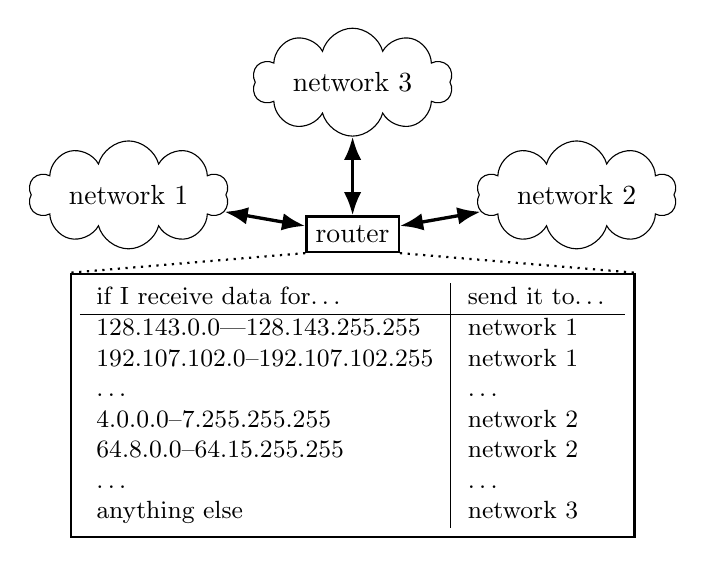
\begin{tikzpicture}
\tikzset{>=Latex},
\node[draw,thick] (router) {router};
\node[aspect=3,draw,cloud,anchor=east,minimum width=2.5cm] (network 1) at ([xshift=-1cm,yshift=.5cm] router.west) {
    network 1
};
\node[aspect=3,draw,cloud,anchor=west,minimum width=2.5cm] (network 2) at ([xshift=1cm,yshift=.5cm] router.east) {
    network 2
};
\node[aspect=3,draw,cloud,anchor=south,minimum width=2.5cm] (network 3) at ([yshift=1cm] router.north) {
    network 3
};
\foreach \x in {1,2,3} { \draw[<->,very thick] (router) -- (network \x); }
\node[anchor=north,font=\small,draw,thick] (table) at ([yshift=-.25cm]router.south) {
\begin{tabular}{l|l}
if I receive data for\ldots & send it to\ldots \\ \hline
128.143.0.0---128.143.255.255 & network 1 \\
192.107.102.0--192.107.102.255 & network 1 \\
\ldots & \ldots \\
4.0.0.0--7.255.255.255 & network 2 \\
64.8.0.0--64.15.255.255 & network 2 \\
\ldots & \ldots \\
anything else & network 3 \\
\end{tabular}
};
\draw[thick,dotted] (router.south west) -- (table.north west);
\draw[thick,dotted] (router.south east) -- (table.north east);
\end{tikzpicture}
\end{frame}




\subsection{special addresses}
\begin{frame}{selected special IPv4 addresses}
\begin{itemize}
\item 127.0.0.0 --- 127.255.255.255 --- localhost
    \begin{itemize}
    \item AKA loopback
    \item the machine we're on
    \item typically only 127.0.0.1 is used
    \end{itemize}
\item 192.168.0.0--192.168.255.255 and \\ 10.0.0.0--10.255.255.255 and \\ 172.16.0.0--172.31.255.255 
    \begin{itemize}
    \item ``private'' IP addresses
    \item not used on the Internet
    \item commonly connected to Internet with \myemph{network address translation}
    \item also 100.64.0.0--100.127.255.255 (but with restrictions)
    \end{itemize}
\item 169.254.0.0-169.254.255.255
    \begin{itemize}
    \item link-local addresses --- `never' forwarded by routers
    \end{itemize}
\end{itemize}
\end{frame}



\section{TCP/UDP}
\againframe<6>{layerOverview}

\subsection{port numbers}
\begin{frame}{port numbers}
    \begin{itemize}
    \item we run multiple programs on a machine
        \begin{itemize}
        \item IP addresses identifying machine --- not enough
        \end{itemize}
    \item<2-> so, add 16-bit \textit{port numbers}
        \begin{itemize}
        \item<2-> think: multiple PO boxes at address
        \end{itemize}
    \vspace{.5cm}
    \item<3-> 0--49151: typically assigned for particular services
        \begin{itemize}
        \item 80 = http, 443 = https, 22 = ssh, \ldots
        \end{itemize}
    \item<3-> 49152--65535: allocated on demand
        \begin{itemize}
        \item default ``return address'' for client connecting to server
        \end{itemize}
    \end{itemize}
\end{frame}



\subsection{UDP v TCP}
\begin{frame}[fragile]{UDP v TCP}
    \begin{itemize}
    \item UDP: messages sent to program, but no reliablity/streams
        \begin{itemize}
        \item \texttt{SOCK\_DGRAM} with socket() instead of \texttt{SOCK\_STREAM}
        \item can sendto()/recvfrom() multiple other programs with one socket
            \begin{itemize}
            \item (but don't have to)
            \end{itemize}
        \item send messages which are limited in size, unreliable
        \end{itemize}
    \item TCP: stream to other program
        \begin{itemize}
        \item need to bind() + listen() + accept() or connect() to setup connection
        \item one socket per connection
        \item read/write bytes --- divided into messages automatically
        \item reliable --- acknowledgments/resending handled for you
        \end{itemize}
    \end{itemize}
\end{frame}


\subsection{OS tracking connections}
\begin{frame}{connections in TCP/IP}
    \begin{itemize}
    \item connection identified by \textit{5-tuple}
        \begin{itemize}
        \item used by OS to lookup ``where is the socket?''
        \end{itemize}
    \item \small(protocol=TCP/UDP, local IP addr., local port, remote IP addr., remote port)
    \vspace{.5cm}
    \item local IP address, port number can be set with \texttt{bind()} function
        \begin{itemize}
        \item \textit{typically} always done for servers, not done for clients
        \item system will choose default if you don't
        \end{itemize}
    \end{itemize}
\end{frame}

\begin{frame}[fragile,label=laptopNetstat]{connections on my desktop}
\begin{lstlisting}[language={},basicstyle=\fontsize{9.5}{10.5}\selectfont]
cr4bd@reiss-t3620>/u/cr4bd
$ netstat --inet --inet6 --numeric
Active Internet connections (w/o servers)
Proto Recv-Q Send-Q Local Address           Foreign Address         State      
tcp        0      0 128.143.67.91:49202     128.143.63.34:22        ESTABLISHED
tcp        0      0 128.143.67.91:803       128.143.67.236:2049     ESTABLISHED
tcp        0      0 128.143.67.91:50292     128.143.67.226:22       TIME_WAIT  
tcp        0      0 128.143.67.91:54722     128.143.67.236:2049     TIME_WAIT  
tcp        0      0 128.143.67.91:52002     128.143.67.236:111      TIME_WAIT  
tcp        0      0 128.143.67.91:732       128.143.67.236:63439    TIME_WAIT  
tcp        0      0 128.143.67.91:40664     128.143.67.236:2049     TIME_WAIT  
tcp        0      0 128.143.67.91:54098     128.143.67.236:111      TIME_WAIT  
tcp        0      0 128.143.67.91:49302     128.143.67.236:63439    TIME_WAIT  
tcp        0      0 128.143.67.91:50236     128.143.67.236:111      TIME_WAIT  
tcp        0      0 128.143.67.91:22        172.27.98.20:49566      ESTABLISHED
tcp        0      0 128.143.67.91:51000     128.143.67.236:111      TIME_WAIT  
tcp        0      0 127.0.0.1:50438         127.0.0.1:631           ESTABLISHED
tcp        0      0 127.0.0.1:631           127.0.0.1:50438         ESTABLISHED
\end{lstlisting}
\end{frame}

\begin{frame}{non-connection sockets}
\begin{itemize}
\item TCP servers waiting for connections + \\
UDP sockets with no particular remote host
\item Linux: OS keeps 5-tuple with ``wildcard'' remote address
\end{itemize}
\end{frame}

\begin{frame}[fragile,label=laptopNetstat]{``listening'' sockets on my desktop}
\begin{lstlisting}[language={},basicstyle=\fontsize{9.5}{10.5}\selectfont]
cr4bd@reiss-t3620>/u/cr4bd
$ netstat --inet --inet6 --numeric --listen
Active Internet connections (only servers)
Proto Recv-Q Send-Q Local Address           Foreign Address         State      
tcp        0      0 127.0.0.1:38537         0.0.0.0:*               LISTEN     
tcp        0      0 127.0.0.1:36777         0.0.0.0:*               LISTEN     
tcp        0      0 0.0.0.0:41099           0.0.0.0:*               LISTEN     
tcp        0      0 0.0.0.0:45291           0.0.0.0:*               LISTEN     
tcp        0      0 127.0.0.1:51949         0.0.0.0:*               LISTEN     
tcp        0      0 127.0.0.1:41071         0.0.0.0:*               LISTEN     
tcp        0      0 0.0.0.0:111             0.0.0.0:*               LISTEN     
tcp        0      0 127.0.0.1:32881         0.0.0.0:*               LISTEN     
tcp        0      0 127.0.0.1:38673         0.0.0.0:*               LISTEN     
....
tcp6       0      0 :::42689                :::*                    LISTEN
udp        0      0 128.143.67.91:60001     0.0.0.0:*
udp        0      0 128.143.67.91:60002     0.0.0.0:*
...
udp6       0      0 :::59938                :::* 
\end{lstlisting}
\end{frame}


\section{DNS}
\againframe<2>{nameAndAddr}
\usetikzlibrary{arrows.meta,positioning,shapes.callouts}
\begin{frame}[fragile,label=dnsDD]{DNS: distributed database}
\begin{tikzpicture}
    \tikzset{
        >=Latex,
        comp box/.style={draw, thick, align=center, minimum width=1.5cm,minimum height=1.5cm},
        explain box/.style={draw=red,very thick, align=left},
        msg/.style={font=\small},
        cmd/.style={font=\small},
        my callout2/.style={draw,fill=blue!10!white,rectangle callout,callout absolute pointer=(#1),below right=5pt of {#1}}
    }
    \node[comp box] (my machine) at (0, 0) { my \\ machine };
    \node[comp box] (isp) at (6, 0) { ISP's \\ DNS server };
    \begin{visibleenv}<1>
        \node[my callout2=isp.south,fill=red!10,align=center,font=\small,anchor=north] at ([xshift=-2cm,yshift=-2cm]isp.south) {
            address sent to my machine \\
            when it connected to network
        };
    \end{visibleenv}
    \begin{visibleenv}<3->
    \node[comp box] (root) at (11, 2) { root \\ DNS server };
    \end{visibleenv}
    \begin{visibleenv}<4->
    \node[comp box] (edu) at (11, 0) { .edu \\ DNS server };
    \node[comp box] (virginia) at (11, -2) { virginia.edu \\ DNS server };
    \node[comp box] (cs) at (11, -4) { {\small cs.virginia.edu} \\ DNS server };
    \end{visibleenv}
    \begin{visibleenv}<2->
    \draw[very thick,<->] (my machine) -- (isp)
        coordinate[midway] (midpt);
    \node[my callout2=midpt,anchor=south,font=\fontsize{9}{10}\selectfont,align=left] at ([yshift=1cm]midpt) {
        address for \\ www.cs.virginia.edu?
    };
    \end{visibleenv}
    \begin{visibleenv}<5->
    \node[my callout2=midpt,anchor=north,font=\fontsize{9}{10}\selectfont,align=left] at ([yshift=-1cm]midpt) {
        www.cs.virginia.edu = \\
        128.143.67.11
    };
    \end{visibleenv}
    \foreach \n/\when in {root/3,edu/4,virginia/4,cs/4} {
        \draw[very thick,<->,alt=<\when->{}{invisible}] (isp) -- (\n.west) coordinate[midway] (midpt \n);
    }
    \begin{visibleenv}<3->
        \node[my callout2=midpt root,anchor=south,font=\fontsize{9}{10}\selectfont,align=left,
              alt=<5>{fill=red!10}] at ([yshift=1cm]midpt root) {
            www.cs.virginia.edu? \\
            try .edu server at \ldots
        };
        \begin{visibleenv}<5>
            \draw[very thick,dotted,red,<->] (isp) -- (root.west);
            \node[draw=red,very thick,fill=white,align=left,anchor=north,font=\small] at ([yshift=-3cm]midpt root) {
                .edu server doesn't change much \\
                optimization: \textit{cache} its address \\
                ~ \\
                check for updated version once in a while
            };
        \end{visibleenv}
    \end{visibleenv}
\end{tikzpicture}
\end{frame}


\subsection{URLs and URIs}
\begin{frame}{URL / URIs}
\begin{itemize}
\item Uniform Resource Locators (URL)
    \begin{itemize}
    \item tells how to find ``resource'' on network
    \end{itemize}
\item Unifrom Resources Identifiers
    \begin{itemize}
    \item superset of URLs
    \end{itemize}
\end{itemize}
\end{frame}

\begin{frame}[fragile]{URI examples}
\begin{Verbatim}[fontsize=\small]
https://kytos02.cs.virginia.edu:443/cs3130-spring2023/
                quizzes/quiz.php?qid=02#q2

https://kytos02.cs.virginia.edu/cs3130-spring2023/
                quizzes/quiz.php?qid=02

https://www.cs.virginia.edu/

sftp://cr4bd@portal.cs.virginia.edu/u/cr4bd/file.txt

tel:+1-434-982-2200
\end{Verbatim}
\end{frame}


\begin{frame}[fragile]{URI generally}
\begin{Verbatim}
scheme://authority/path?query#fragment
\end{Verbatim}
\begin{itemize}
\item scheme: --- what protocol
\item //authority/
    \begin{itemize}
    \item authoirty = user@host:port OR host:port OR user@host OR host
    \end{itemize}
\item path
    \begin{itemize}
    \item which resource
    \end{itemize}
\item ?query --- usually key/value pairs 
\item \#fragment --- place in resource
\vspace{.5cm}
\item most components (sometimes) optional
\end{itemize}
\end{frame}



\section{DHCP and IPv6 autoconfig}

\begin{frame}{autoconfiguration}
\begin{itemize}
\item problem: how does my machine get IP address
\vspace{.5cm}
\item otherwise:
    \begin{itemize}
    \item have sysadmin type one in?
    \item just choose one?
    \item \myemph<2>{ask machine on local network to assign it}
    \end{itemize}
\vspace{.5cm}
\item<3-> often local router machine runs service to assign IP addresses
    \begin{itemize}
    \item knows what IP addresses are available
    \item sysadmin might configure in mapping from MAC addresses to IP addresses
    \end{itemize}
\end{itemize}
\end{frame}

\begin{frame}{DHCP high-level}
    \begin{itemize}
    \item protocol done over UDP
    \vspace{.5cm}
    \item but since we don't have IP address yet, use \texttt{0.0.0.0}
    \item and since we don't know server address, use \texttt{255.255.255.255}
        \begin{itemize}
        \item = ``everyone on the local network''
        \end{itemize}
    \item local server replies to request with address + \myemph<2>{time limit}
    \item later: can send messages to local server to renew/give up address
    \end{itemize}
\end{frame}

\begin{frame}{exercise: why time limit?}
    \begin{itemize}
        \item DHCP ``lease''
        \item rather than getting address forever
        \vspace{.5cm}
        \item but DHCP has way of releasing taken address
        \vspace{.5cm}
        \item why impose a time limit
    \end{itemize}
\end{frame}



\section{NAT}
\begin{frame}{network address translation}
\begin{itemize}
\item IPv4 addresses are kinda scarce
\item solution: \textit{convert} many private addrs. to one public addr.
\item locally: use private IP addresses for local addresses
\item outside: private IP addresses become a single public one
\item commonly how home networks work (and some ISPs)
\end{itemize}
\end{frame}

\begin{frame}{NAT idea}
\begin{tikzpicture}
\tikzset{network/.style={draw,very thick,cloud,aspect=2}}
\node[align=center,network] (outside) at (0, 0){external};
\node[draw,very thick,minimum height=2cm,align=center](router) at (5, 0) {
    router \\
    {\fontsize{9}{10}\tt 203.0.113.43} \\
    {\fontsize{9}{10}\tt 192.168.1.1} 
};
\node[align=center,network] (inside) at (9.5, 0){internal\\\fontsize{9}{10}\tt 192.168.1.*};
\foreach \x/\v in {2/2, 1/3, 0/4, -1/5, -2/6} {
    \node[draw,very thick,circle,
        label={[overlay,font=\fontsize{8}{9}\selectfont]right:192.168.1.\v}
    ] (i-\x) at (12, \x) {};
    \draw (inside) -- (i-\x);
}
\begin{pgfonlayer}{bg}
\begin{scope}[line width=1mm,black!50]
    \draw (outside) -- (router);
    \draw (router) -- (inside);
\end{scope}
\end{pgfonlayer}
\tikzset{
    box/.style={draw,ultra thick,align=center,fill=white,font=\fontsize{13}{14}\selectfont}
}
\node[box] (before) at ([yshift=-3cm]$(outside.east)!0.3!(router)$) {
    1.2.3.4:443 \\ $\rightarrow$ \\ \myemph{203.0.113.43}:54923
};
\node[box] (after) at ([yshift=-3cm]$(router)!0.8!(inside.west)$) {
    1.2.3.4:443 \\ $\rightarrow$ \\ \myemph{192.168.1.4}:39129
};
\draw[dotted,thick] (before.north) -- (before.north |- outside.east);
\draw[dotted,thick] (after.north) -- (after.north |- outside.east);

\end{tikzpicture}
\end{frame}


\begin{frame}{NAT illusion}
    \begin{itemize}
    \item NAT illusion:
    \item private IP address communicating directly with public IP
    \vspace{.5cm}
    \item inside network, talking to outside:
        \begin{itemize}
        \item use private local address
        \item use public remote address
        \item never see router's address
        \end{itemize}
    \item outside network, talking to inside
        \begin{itemize}
        \item use public local address
        \item use router's public address
        \end{itemize}
    \end{itemize}
\end{frame}

\begin{frame}{implementing NAT}
\small
\begin{tabular}{llll}
remote host + port & outside local port number & inside IP & inside port number \\ \hline
128.148.17.3:443 & 54033 & 192.168.1.5 & 43222 \\
11.7.17.3:443 & 53037 & 192.168.1.5 & 33212 \\
128.148.31.2:22 & 54032 & 192.168.1.37 & 43010 \\
128.148.17.3:443 & 63039 & 192.168.1.37 & 32132 \\
\end{tabular}
\begin{itemize}
\item table of the translations
\item need to update as new connections made
\end{itemize}
\end{frame}


\section{lab API}
\begin{frame}{upcoming lab}
    \begin{itemize}
    \item receive message split into pieces
    \item you are responsible for:
        \begin{itemize}
        \item requesting parts in order
        \item resending requests if messages lost/corrupted
        \end{itemize}
    \item ``acknowledge'' receiving part X to request part X+1
    \end{itemize}
\end{frame}

\begin{frame}{protocol}
    \begin{itemize}
    \item GET0 --- start
        \begin{itemize}
        \item other end acknowledges by giving data
        \item if they don't acknowledge, you need to send again
        \end{itemize}
    \item ACKn 
        \begin{itemize}
        \item request message n + 1 by acknowledging message n
        \item not quite same purpose as acknowledgments in lecture examples
        \item (in lab, the respoonse is your `acknowledgment' of your request; \\
            you retry if you don't get it)
        \end{itemize}
    \end{itemize}
\end{frame}


\begin{frame}[fragile]{callback-based programming (1)}
\begin{Verbatim}[fontsize=\small]
/* library code you don't write */
void mainLoop() {
    while (true) {
        Event event = getNextEvent();
        if (event.type == RECIEVED) {
            recvd(...);
        } else if (event.type == TIMEOUT) {
            (event.timeout_function)(...);
        }
        ...
    }
}
\end{Verbatim}
\end{frame}

\begin{frame}[fragile]{callback-based programming (2)}
\begin{Verbatim}[fontsize=\small]
/* your code, called by library */
void recvd(...) {
    ...
    setTimeout(..., timerCallback, ...);
}

void timerCalback(...) {
    ...
}
\end{Verbatim}
\end{frame}

\begin{frame}{callback-based programming}
    \begin{itemize}
    \item writing scripts in a webpage
    \item many graphical user interface libraries
    \item sometimes servers that handle lots of connections
    \end{itemize}
\end{frame}

